\chapter{Introduction}

Let me introduce to the topic of my PhD work at \acrfull{sk}.

\todo[inline]{TODO: complete chapter}

\section{Thesis Structure}
The diagram in \autoref{fig:thesis-structure} illustrates the flow of information through the structure of the thesis.

\begin{figure}[htb!]
\centering 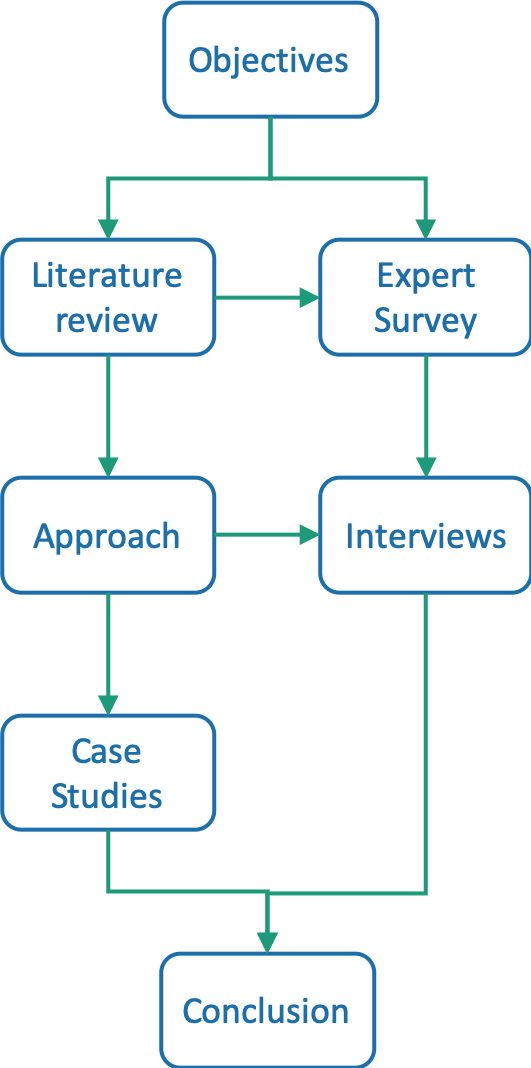
\includegraphics[width=0.5\textwidth]{graphics/thesis-structure}
\caption{Thesis structure}
\label{fig:thesis-structure}
\end{figure}

\begin{description}
    \item[\Autoref{cap:background} - Background]
Here's the literature review.

    \item[\Autoref{cap:thesis_objectives} - Thesis Objectives]
We define the objectives of our work.

...

    \item[\Autoref{cap:conclusion} - Conclusion]
In the last chapter, we discuss our results obtained ...

\end{description}

